% !TeX program = lualatex
\documentclass[12pt, a4paper]{article}
\usepackage{fullpage}
\usepackage{subfiles}
\usepackage{fontspec}
\usepackage{libertine}
\usepackage{xcolor}
\usepackage{GotIn}
\usepackage{geometry}
\usepackage{multicol}
\usepackage{multicolrule}
\usepackage{graphicx}
\usepackage{enumitem}
\usepackage[autocompile]{gregoriotex}
\usepackage[latin,french]{babel}


\geometry{top=2cm, bottom=2cm}
% \pagestyle{empty}

\definecolor{red}{HTML}{C70039}
% \input GoudyIn.fd
% \newcommand*\initfamily{\usefont{U}{GoudyIn}{xl}{n}}

\input Acorn.fd
\newcommand*\initfamily{\usefont{U}{Acorn}{xl}{n}}
% cette ligne ajoute de l'espace entre les portées
% \grechangedim{baselineskip}{60pt}{scalable}

\begin{document}
  \gresetlinecolor{gregoriocolor}

  \begin{titlepage}\centering
    \vspace*{\fill}\
    \huge Secondes Vêpres\\
    \smallskip
    \begin{Large}
      \textit{
        Fête-Dieu\\
      }
    \end{Large}
    \medskip
    \large et\\
    \medskip
    \LARGE Salut du Saint-Sacrement\\
    \bigskip
    % \begin{figure}[h!]
    %   \centering
    %   
\includegraphics[width=7cm]{../ordinaires/logo.png}
    % \end{figure}
    \vspace*{\fill}
    \begin{figure}[h!]
      \centering
      
\includegraphics[width=7cm]{../ordinaires/logo.png}
    \end{figure}
    \centering \normalsize Paroisse Saint Roch\\
    \bigskip
    \begin{Large}
      \centering Ne pas emporter
    \end{Large}
  \end{titlepage}

  \newpage
  \vspace*{\fill}
    \begin{center}
      \normalsize\textit{
        Livret latin-français
      }
    \end{center}
  \newpage

  \begin{center}
    \textcolor{red}{\large{Ouverture.}}
  \end{center}

  % greillumination: remplace la première lettre, ici par une font ornementale
  \greillumination{\initfamily\fontsize{11mm}{11mm}\selectfont D}
  \gregorioscore{../ordinaires/vepres-deus_in_adjutorium}

  \begin{center}
    \small{
    \emph{
      Dieu, venez à mon aide ; Seigneur, hatez-vous de me secourir.\\
      Gloire au Père, au Fils et au Saint Esprit, comme il était au commencement, maintenant et toujour et dans les siècles des siècles. Allelúia\\
    }
  }
  \end{center}

  \newpage
  \normalsize

  % ===== DEBUT Antienne =========
  \gresetinitiallines{1}
  \greillumination{\initfamily\fontsize{11mm}{11mm}\selectfont S}
  \gregorioscore{antiennes/an--sacerdos_in_aeternum--solesmes_1961}
  \begin{center}
    \footnotesize{
      \textit{Prêtre pour l’éternité selon l’ordre de Melchisédech, le Christ Seigneur a offert le pain et le vin.}
    }
  \end{center}
  % ===== FIN Antienne ===========

  % ===== DEBUT psaume ===========
  % gresetinitiallines : avec le parametre à 0, supprime l'ornement
  \begin{center}
    \large{Psaume 109.}\\
  \end{center}

  \gresetinitiallines{0}
  \gregorioscore{psaumes/psaume109-If}

  \begin{enumerate}[label=\textcolor{red}{\arabic*}]
    \setcounter{enumi}{1}
    \item Donec ponam ini\textbf{mí}cos \textbf{tu}os,\textcolor{red}{~*} scabéllum pe\textit{dum} \textit{tu}\textbf{ó}rum.

    \item Virgam virtútis tuæ emíttet Dómi\textbf{nus} ex \textbf{Si}on:\textcolor{red}{~*} domináre in médio inimicó\textit{rum} \textit{tu}\textbf{ó}rum.

    \item Tecum princípium in die virtútis tuæ in splendóri\textbf{bus} sanc\textbf{tó}rum:\textcolor{red}{~*} ex útero ante lucíferum \textit{gé}\textit{nu}\textbf{i} te.

    \item Jurávit Dóminus, et non pœni\textbf{té}bit \textbf{e}um:\textcolor{red}{~*} Tu es sacérdos in ætérnum secúndum órdi\textit{nem} \textit{Mel}\textbf{chí}sedech.

    \item Dóminus a \textbf{dex}tris \textbf{tu}is,\textcolor{red}{~*} confrégit in die iræ \textit{su}\textit{æ} \textbf{re}ges.

    \item Judicábit in natiónibus, im\textbf{plé}bit ru\textbf{í}nas:\textcolor{red}{~*} conquassábit cápita in ter\textit{ra} \textit{mul}\textbf{tó}rum.

    \item De torrénte in \textbf{vi}a \textbf{bi}bet:\textcolor{red}{~*} proptérea exal\textit{tá}\textit{bit} \textbf{ca}put.

    \item Glória \textbf{Pa}tri, et \textbf{Fí}lio,\textcolor{red}{~*} et Spirí\textit{tu}\textit{i} \textbf{Sanc}to.

    \item Sicut erat in princípio, et \textbf{nunc}, et \textbf{sem}per,\textcolor{red}{~*} et in sǽcula sæcu\textit{ló}\textit{rum}. \textbf{A}men.
  \end{enumerate}
  %  Répetition de l'Antienne
  \grecommentary{\textit{Reprise de l'Antienne.}}
  \gabcsnippet{(c4) SA(df)cér(d)dos(dc) in(f) ae(g)tér(f_h)num(h.) <c>*</c>(,) Chri(h_j)stus(hvGF') Dó(g)mi(gh)nus(h.) (;) se(h)cún(h_j!kvJH'i)dum(h') ór(h)di(h)nem(hg) Mel(h)chí(gf)se(gh)dech,(h.) (;) pa(f)nem(gh) et(g) vi(fe)num(fgf') ób(d)tu(cd)lit.(d.) (::) }

  \newpage
  \vspace*{\fill}\
  \begin{normalsize}
    \begin{center}
      \par \textit{Prêtre pour l’éternité selon l’ordre de Melchisédech, le Christ Seigneur a offert le pain et le vin. }
      \medskip
      \begin{enumerate}[label=\textcolor{red}{\emph{\arabic*}}]
        \item \textit{Le Seigneur a dit à mon Seigneur : Asseyez-toi à ma droite, }
        \item \textit{Jusqu'à ce que je mette tes ennemis pour le marchepied de tes pieds.}
        \item \textit{L'Éternel enverra de Sion la verge de ta force: Domine au milieu de tes ennemis!}
        \item \textit{Ton peuple sera un peuple de franche volonté, au jour de ta puissance, en sainte magnificence. Du sein de l'aurore te viendra la rosée de ta jeunesse.}
        \item \textit{L'Éternel a juré, et il ne se repentira point: Tu es sacrificateur pour toujours, selon l'ordre de Melchisédec.}
        \item \textit{Le Seigneur, à ta droite, brisera les rois au jour de sa colère.}
        \item \textit{Il jugera parmi les nations, il remplira tout de corps morts, il brisera le chef d'un grand pays.}
        \item \textit{Il boira du torrent dans le chemin, c'est pourquoi il lèvera haut la tête.}
        \item \textit{Gloire au Père, au Fils, et au Saint Esprit, }
        \item \textit{Comme il était au commencement, maintenant et toujours, et dans les siècles des siècles. Amen. }
      \end{enumerate}
    \end{center}
  \end{normalsize}
  \vspace*{\fill}\
  \newpage

  % ===== DEBUT Antienne =========
  \gresetinitiallines{1}
  \greillumination{\initfamily\fontsize{11mm}{11mm}\selectfont M}
  \gregorioscore{antiennes/an--miserator_dominus--solesmes_1961}
  \begin{center}
    \footnotesize{
      \textit{Le Seigneur miséricordieux et indulgent a nourri ceux qui le craignent, en mémoire de ses merveilles.}
    }
  \end{center}
  % ===== FIN Antienne ===========

  % ===== DEBUT psaume ===========
  % gresetinitiallines : avec le parametre à 0, supprime l'ornement
  \begin{center}
    \large{Psaume 110.}\\
  \end{center}

  \gresetinitiallines{0}
  \gregorioscore{psaumes/psaume110-IID}

  \begin{enumerate}[label=\textcolor{red}{\arabic*}]
    \setcounter{enumi}{1}
    \item Magna ópera \textbf{Dó}mini:\textcolor{red}{~*} exquisíta in omnes voluntá\textit{tes} \textbf{e}jus.

    \item Conféssio et magnificéntia opus \textbf{e}jus:\textcolor{red}{~*} et justítia ejus manet in sǽcu\textit{lum} \textbf{sǽ}culi.

    \item Memóriam fecit mirabílium suórum,\textcolor{red}{~†}  miséricors et miserátor \textbf{Dó}minus:\textcolor{red}{~*} escam dedit timén\textit{ti}\textbf{bus} se.

    \item Memor erit in sǽculum testaménti \textbf{su}i:\textcolor{red}{~*} virtútem óperum suórum annuntiábit pópu\textit{lo} \textbf{su}o:

    \item Ut det illis hereditátem \textbf{gén}tium:\textcolor{red}{~*} ópera mánuum ejus véritas, et \textit{ju}\textbf{dí}cium.

    \item Fidélia ómnia mandáta ejus:\textcolor{red}{~†}  confirmáta in sǽculum \textbf{sǽ}culi,\textcolor{red}{~*} facta in veritáte et æ\textit{qui}\textbf{tá}te.

    \item Redemptiónem misit pópulo \textbf{su}o:\textcolor{red}{~*} mandávit in ætérnum testamén\textit{tum} \textbf{su}um.

    \item Sanctum, et terríbile nomen \textbf{e}jus:\textcolor{red}{~*} inítium sapiéntiæ ti\textit{mor} \textbf{Dó}mini.

    \item Intelléctus bonus ómnibus faciéntibus \textbf{e}um:\textcolor{red}{~*} laudátio ejus manet in sǽcu\textit{lum} \textbf{sǽ}culi.

    \item Glória Patri, et \textbf{Fí}lio,\textcolor{red}{~*} et Spirítu\textit{i} \textbf{Sanc}to.

    \item Sicut erat in princípio, et nunc, et \textbf{sem}per,\textcolor{red}{~*} et in sǽcula sæculó\textit{rum}. \textbf{A}men.
  \end{enumerate}
  %  Répetition de l'Antienne
  \grecommentary{\textit{Reprise de l'Antienne.}}
  \gabcsnippet{(f3) Mi(c)se(ef)rá(f)tor(fe) Dó(f!gwh_f)mi(ef)nus(f.) (,) e(fj)scam(j) de(ih)dit(gf) ti(g)mén(hi)ti(g)bus(hvGF'E) se(f.) (;) in(jij) me(ih)mó(i)ri(ij)am(j.) (,) su(fh)ó(ge)rum(c) mi(e)ra(fg)bí(h)li(gvFE)um.(f.) (::)}

  \newpage
  \vspace*{\fill}\
  \begin{normalsize}
    \begin{center}
      \par \textit{Le Seigneur miséricordieux et indulgent a nourri ceux qui le craignent, en mémoire de ses merveilles. }
      \medskip
      \begin{enumerate}[label=\textcolor{red}{\emph{\arabic*}}]
        \item \textit{De tout cœur je rendrai grâce au Seigneur dans l'assemblée, parmi les justes.}
        \item \textit{Grandes sont les œuvres du Seigneur ; tous ceux qui les aiment s'en instruisent.}
        \item \textit{Noblesse et beauté dans ses actions : à jamais se maintiendra sa justice.}
        \item \textit{De ses merveilles il a laissé un mémorial ; le Seigneur est tendresse et pitié, il a donné des vivres à ses fidèles,}
        \item \textit{Gardant toujours mémoire de son
        alliance, il a montré sa force à son peuple.}
        \item \textit{Lui donnant le domaine des nations. Justesse et sûreté les œuvres de ses mains.}
        \item \textit{Sécurité, toutes ses lois, établies pour toujours et à jamais, accomplies avec droiture et sûreté ! }
        \item \textit{Il apporte la délivrance à son peuple ; son alliance est promulguée pour toujours.}
        \item \textit{Saint, redoutable est son nom, la sagesse commence avec la crainte du Seigneur.}
        \item \textit{Qui accomplit sa volonté en est éclairé. A jamais se maintiendra sa louange.}
        \item \textit{Gloire au Père, au Fils, et au Saint Esprit, }
        \item \textit{Comme il était au commencement, maintenant et toujours, et dans les siècles des siècles. Amen. }
      \end{enumerate}
    \end{center}
  \end{normalsize}
  \vspace*{\fill}\
  \newpage

  % ===== DEBUT Antienne =========
  \gresetinitiallines{1}
  \greillumination{\initfamily\fontsize{11mm}{11mm}\selectfont C}
  \gregorioscore{antiennes/an--calicem_salutaris_accipiam_et_sacrificabo--solesmes_1961}
  \begin{center}
    \footnotesize{
      \textit{Je prendrai le Calice du salut, et je sacrifierai un sacrifice de louange. }
    }
  \end{center}
  % ===== FIN Antienne ===========

  % ===== DEBUT psaume ===========
  % gresetinitiallines : avec le parametre à 0, supprime l'ornement
  \begin{center}
    \large{Psaume 115.}\\
  \end{center}

  \gresetinitiallines{0}
  \gregorioscore{psaumes/psaume115-IIIa2}

  \begin{enumerate}[label=\textcolor{red}{\arabic*}]
    \setcounter{enumi}{1}
    \item Ego dixi in ex\textbf{cés}su \textbf{me}o:\textcolor{red}{~*} Omnis \textit{ho}\textit{mo} \textbf{men}dax.

    \item Quid re\textbf{trí}buam \textbf{Dó}\textbf{mi}no,\textcolor{red}{~*} pro ómnibus, quæ retrí\textit{bu}\textit{it} \textbf{mi}hi?

    \item Cálicem salu\textbf{tá}ris ac\textbf{cí}\textbf{pi}am:\textcolor{red}{~*} et nomen Dómini \textit{in}\textit{vo}\textbf{cá}bo.

    \item Vota mea Dómino reddam coram omni \textbf{pó}pulo \textbf{e}jus:\textcolor{red}{~*} pretiósa in conspéctu Dómini mors sanc\textit{tó}\textit{rum} \textbf{e}jus:

    \item O Dómine, quia ego \textbf{ser}vus \textbf{tu}us:\textcolor{red}{~*} ego servus tuus, et fílius an\textit{cíl}\textit{læ} \textbf{tu}æ.

    \item Dirupísti víncula mea:\textcolor{red}{~†}  tibi sacrificábo \textbf{hós}tiam \textbf{lau}dis,\textcolor{red}{~*} et nomen Dómini \textit{in}\textit{vo}\textbf{cá}bo.

    \item Vota mea Dómino reddam in conspéctu omnis \textbf{pó}puli \textbf{e}jus:\textcolor{red}{~*} in átriis domus Dómini, in médio tu\textit{i}, \textit{Je}\textbf{rú}salem.

    \item Glória \textbf{Pa}tri, et \textbf{Fí}\textbf{li}o,\textcolor{red}{~*} et Spirí\textit{tu}\textit{i} \textbf{Sanc}to.

    \item Sicut erat in princípio, et \textbf{nunc}, et \textbf{sem}per,\textcolor{red}{~*} et in sǽcula sæcu\textit{ló}\textit{rum}. \textbf{A}men.
  \end{enumerate}
  %  Répetition de l'Antienne
  \grecommentary{\textit{Reprise de l'Antienne.}}
  \gabcsnippet{(c4) Ca(e_[oh:h]d)li(g)cem(hj) (,) sa(ijk)lu(j')tá(j)ris(ji) ac(h)cí(ji)pi(hg)am,(g.) (;) et(gh!ij) sa(h')cri(g)fi(e)cá(fg)bo(g_[uh:l]h) (,) hó(hvGF')sti(g)am(gf) lau(e.)dis.(e.) (::)}

  \newpage
  \vspace*{\fill}\
  \begin{normalsize}
    \begin{center}
      \par \textit{Je prendrai le Calice du salut, et je sacrifierai un sacrifice de louange.}
      \medskip
      \begin{enumerate}[label=\textcolor{red}{\emph{\arabic*}}]
        \item \textit{J’ai cru, c’est pourquoi j’ai parlé : je suis dans une humiliation extrême.}
        \item \textit{J’ai dit dans l’excès de ma douleur : Tout homme est menteur.}
        \item \textit{Que rendrai-je au Seigneur, pour tous les biens qu’il m’a faits ?}
        \item \textit{Je prendrai le Calice du salut, et j’invoquerai le nom du Seigneur. }
        \item \textit{Je rendrai mes vœux au Seigneur en présence de tout son peuple : précieuse est la mort de ses Saints aux yeux du Seigneur.}
        \item \textit{O Seigneur, parce que je suis ton serviteur, et le fils de ta servante. }
        \item \textit{Tu as brisé mes liens : je te sacrifierai un sacrifice de louange, et j’invoquerai le nom du Seigneur.}
        \item \textit{Je rendrai mes vœux au Seigneur devant tout son peuple ; dans le vestibule de la maison du Seigneur, au milieu de toi, ô Jérusalem. }
        \item \textit{Gloire au Père, au Fils, et au Saint Esprit, }
        \item \textit{Comme il était au commencement, maintenant et toujours, et dans les siècles des siècles. Amen. }
      \end{enumerate}
    \end{center}
  \end{normalsize}
  \vspace*{\fill}\
  \newpage

  % ===== DEBUT Antienne =========
  \gresetinitiallines{1}
  \greillumination{\initfamily\fontsize{11mm}{11mm}\selectfont S}
  \gregorioscore{antiennes/an--sicut_novellae_olivarum--solesmes}
  \begin{center}
    \footnotesize{
      \textit{Comme de nouveaux plants d’olivier, qu’ainsi soient les fils de l’Eglise autour de la table du Seigneur.}
    }
  \end{center}
  % ===== FIN Antienne ===========

  % ===== DEBUT psaume ===========
  % gresetinitiallines : avec le parametre à 0, supprime l'ornement
  \begin{center}
    \large{Psaume 127.}\\
  \end{center}

  \gresetinitiallines{0}
  \gregorioscore{psaumes/psaume127-IVE}

  \begin{enumerate}[label=\textcolor{red}{\arabic*}]
    \setcounter{enumi}{1}
    \item Labóres mánuum tuárum quia \textit{man}\textit{du}\textbf{cá}bis:\textcolor{red}{~*} beátus es, et be\textit{ne} \textit{ti}\textit{bi} \textbf{e}rit.

    \item Uxor tua sicut vi\textit{tis} \textit{ab}\textbf{ún}dans:\textcolor{red}{~*} in latéri\textit{bus} \textit{do}\textit{mus} \textbf{tu}æ.

    \item Fílii tui sicut novéllæ \textit{o}\textit{li}\textbf{vá}rum:\textcolor{red}{~*} in circúi\textit{tu} \textit{men}\textit{sæ} \textbf{tu}æ.

    \item Ecce sic benedi\textit{cé}\textit{tur} \textbf{ho}mo,\textcolor{red}{~*} \textit{qui} \textit{ti}\textit{met} \textbf{Dó}\textbf{mi}num.

    \item Benedícat tibi Dómi\textit{nus} \textit{ex} \textbf{Si}on:\textcolor{red}{~*} et vídeas bona Jerúsalem ómnibus dié\textit{bus} \textit{vi}\textit{tæ} \textbf{tu}æ.

    \item Et vídeas fílios filió\textit{rum} \textit{tu}\textbf{ó}rum:\textcolor{red}{~*} pa\textit{cem} \textit{su}\textit{per} \textbf{Is}\textbf{ra}ël.

    \item Glória Pa\textit{tri}, \textit{et} \textbf{Fí}lio,\textcolor{red}{~*} et Spi\textit{rí}\textit{tu}\textit{i} \textbf{Sanc}to.

    \item Sicut erat in princípio, et \textit{nunc}, \textit{et} \textbf{sem}per,\textcolor{red}{~*} et in sǽcula sæ\textit{cu}\textit{ló}\textit{rum}. \textbf{A}men.
  \end{enumerate}
  %  Répetition de l'Antienne
  \grecommentary{\textit{Reprise de l'Antienne.}}
  \gabcsnippet{(c4) Si(ffe)cut(d) no(f)vél(gh)lae(gf) o(gh)li(gf)vá(e)rum,(e.) (;) Ec(e)clé(g!hi)si(h)ae(h') fí(h)li(gf)i(gh) sint(gv_FE.) (;) in(fe) cir(de)cú(e)i(dc)tu(c) men(gf)sae(ghg) Dó(fe)mi(de)ni.(e.) (::)}

  \newpage
  \vspace*{\fill}\
  \begin{normalsize}
    \begin{center}
      \par \textit{Comme de nouveaux plants d’olivier, qu’ainsi soient les fils de l’Eglise autour de la table du Seigneur.}
      \medskip
      \begin{enumerate}[label=\textcolor{red}{\emph{\arabic*}}]
        \item \textit{Heureux tous ceux qui craignent le Seigneur et qui marchent dans ses voies.}
        \item \textit{Tu mangeras et sera nourri du travail de tes mains ; tu seras heureux et comblé de biens. }
        \item \textit{Ta femme sera comme une vigne féconde dans l’enceinte de ta maison. }
        \item \textit{Tes enfants, comme de nouveaux plants d’oliviers, entoureront ta table.}
        \item \textit{Ainsi sera béni l’homme qui craint le Seigneur.}
        \item \textit{Que le Seigneur te bénisse de Sion ; qu’il te fasse voir Jérusalem dans sa félicité tous les jours de ta vie.}
        \item \textit{Qu’il te fasse voir les enfants de tes enfants ; que la paix soit sur Israël.}
        \item \textit{Gloire au Père, au Fils, et au Saint Esprit, }
        \item \textit{Comme il était au commencement, maintenant et toujours, et dans les siècles des siècles. Amen. }
      \end{enumerate}
    \end{center}
  \end{normalsize}
  \vspace*{\fill}\
  \newpage

  % ===== DEBUT Antienne =========
  \gresetinitiallines{1}
  \greillumination{\initfamily\fontsize{11mm}{11mm}\selectfont Q}
  \gregorioscore{antiennes/an--qui_pacem_ponit--solesmes_1961}
  \begin{center}
    \footnotesize{
      \textit{Celui qui a établi la paix aux enceintes de l’Eglise, c’est le Seigneur, qui nous rassasie du plus pur froment. }
    }
  \end{center}
  % ===== FIN Antienne ===========

  % ===== DEBUT psaume ===========
  % gresetinitiallines : avec le parametre à 0, supprime l'ornement
  \begin{center}
    \large{Psaume 147.}\\
  \end{center}

  \gresetinitiallines{0}
  \gregorioscore{psaumes/psaume147-Va}

  \begin{enumerate}[label=\textcolor{red}{\arabic*}]
    \setcounter{enumi}{1}
    \item Quóniam confortávit seras portárum tu\textbf{á}rum:\textcolor{red}{~*} benedíxit fíliis \textbf{tu}is \textbf{in} te.

    \item Qui pósuit fines tuos \textbf{pa}cem:\textcolor{red}{~*} et ádipe fruménti \textbf{sá}ti\textbf{at} te.

    \item Qui emíttit elóquium suum \textbf{ter}ræ:\textcolor{red}{~*} velóciter currit \textbf{ser}mo \textbf{e}jus.

    \item Qui dat nivem sicut \textbf{la}nam:\textcolor{red}{~*} nébulam sicut \textbf{cí}nerem \textbf{spar}git.

    \item Mittit crystállum suam sicut buc\textbf{cél}las:\textcolor{red}{~*} ante fáciem frígoris ejus quis \textbf{sus}ti\textbf{né}bit?

    \item Emíttet verbum suum, et liquefáciet \textbf{e}a:\textcolor{red}{~*} flabit spíritus ejus, et \textbf{flu}ent \textbf{a}quæ.

    \item Qui annúntiat verbum suum \textbf{Ja}cob:\textcolor{red}{~*} justítias, et judícia \textbf{su}a \textbf{Is}raël.

    \item Non fecit táliter omni nati\textbf{ó}ni:\textcolor{red}{~*} et judícia sua non manifes\textbf{tá}vit \textbf{e}is.

    \item Glória Patri, et \textbf{Fí}lio,\textcolor{red}{~*} et Spi\textbf{rí}tui \textbf{Sanc}to.

    \item Sicut erat in princípio, et nunc, et \textbf{sem}per,\textcolor{red}{~*} et in sǽcula sæcu\textbf{ló}rum. \textbf{A}men.
  \end{enumerate}
  %  Répetition de l'Antienne
  \grecommentary{\textit{Reprise de l'Antienne.}}
  \gabcsnippet{(c3) Qui(d_f) pa(h)cem(fh/iih) (,)  po(h_0i'k)nit(j') fi(i)nes(h') Ec(gxg)clé(hih')si(f)ae,(f.) (;) fru(gxfgh)mén(gf~)ti(e') á(f)di(e)pe(d'_) (,) sá(d!f'h)ti(hi)at(hgh) nos(d.) Dó(ef)mi(ed)nus.(d.) (::)}

  \newpage
  \vspace*{\fill}\
  \begin{normalsize}
    \begin{center}
      \par \textit{Celui qui a établi la paix aux enceintes de l’Eglise, c’est le Seigneur, qui nous rassasie du plus pur froment.}
      \medskip
      \begin{enumerate}[label=\textcolor{red}{\emph{\arabic*}}]
        \item \textit{Loue, Jérusalem, le Seigneur ; loue ton Dieu, Sion.}
        \item \textit{Car c’est lui qui a fortifié tes portes, et qui a béni tes fils au milieu de toi ;}
        \item \textit{Qui a établi la paix dans tes frontières, et qui te rassasie du plus pur froment. }
        \item \textit{Qui envoie sa Parole à la terre, et son Verbe avec promptitude. }
        \item \textit{Qui fait tomber la neige comme de la laine, et répand le brouillard comme de la cendre. }
        \item \textit{Il durcit les eaux, et en forme des glaçons ; et alors qui peut soutenir la rigueur du froid ? }
        \item \textit{A sa Parole la glace se fond ; son Esprit souffle, et les eaux coulent.}
        \item \textit{Il annonce son Verbe à Jacob, ses jugements et ses ordonnances à Israël. }
        \item \textit{Il n’a pas ainsi traité les autres nations ; et il ne leur a pas fait connaître ses jugements. }
        \item \textit{Gloire au Père, au Fils, et au Saint Esprit, }
        \item \textit{Comme il était au commencement, maintenant et toujours, et dans les siècles des siècles. Amen. }
      \end{enumerate}
    \end{center}
  \end{normalsize}
  \vspace*{\fill}\
  \newpage

  \begin{center}
    \textcolor{red}{\large{Capitule}}\\
    \small\textit{
      I\textsuperscript{e} Épître aux Corinthiens. 2, 23-24.
    }
  \end{center}

  \begin{multicols}{2}
    \parindent=0pt
    Fratres : Ego enim accepi a Dómino quod et trádidi vobis, \textcolor{red}{†} quóniam Dóminus Jesus, in qua nocte tradebátur, accépit panem, et grátias agens fregit, et dixit : Accípite, et manducáte : hoc est corpus meum, quod pro vobis tradétur : \textcolor{red}{*} hoc fácite in meam commemoratiónem. \\
    \textcolor{red}{\Rbar.} Deo grátias.

    \columnbreak

    \textit{Frères : c’est du Seigneur lui-même que j’ai appris ce que je vous ai transmis : que le Seigneur Jésus, la nuit où il fut livré, prit du pain, et après avoir rendu grâces, le rompit et dit : Recevez et mangez ; ceci est mon corps qui sera livré pour vous ; faites ceci en mémoire de moi.\\
    \textcolor{red}{\Rbar.} Rendons grâce à Dieu.
    }
  \end{multicols}

  \bigskip

  \begin{center}
    \textcolor{red}{\large{Hymne}}\\
  \end{center}
  
  \gresetinitiallines{1}
  \greillumination{\initfamily\fontsize{11mm}{11mm}\selectfont P}
  \gregorioscore{hymnes/hy--pange_lingua..._corporis--solesmes}
  \begin{multicols}{2}
    \begin{footnotesize}
      \begin{enumerate}[label=\textcolor{red}{\emph{\arabic*}}]
        \item \textit{Chante, ô ma langue, le mystère de la glorieuse chair ; du sang précieux qu'à versé, pour la rançon du monde, le Roi des nations, fruit béni de l'illustre Vierge.}
        \item \textit{Ce roi se donne à nous ; le Verbe né du Père, Nait pour nous d’une Vierge mère : Et parmi les mortels, mortel passe ses jours : Il sème dans les cœurs sa parole féconde ; Et près de partir de ce monde, Par un ordre admirable il achève son cours.}
        \item \textit{Assis avec les siens, la nuit qui fut suivie De la triste fin de sa vie, Il accomplit la loi dans ce dernier festin, En mangeant de l’agneau la Pâque désirée, A ceux de la troupe sacrée, Se donne, en pain vivant, lui-même de sa main.}
        \item \textit{Du Verbe, rendu chair, la parole ineffable Rend le pain sa chair véritable, Et le vin se transforme au sang de notre roi ; Et quoique tous les sens combattent ce mystère, Pour affermir un cœur sincère Il suffit de l’armer d’une invincible foi. }
        \item \textit{Adorons avec crainte au pied de cette table, Un sacrement si vénérable ; Et que l’ancienne loi cède aux nouveaux présents, Que la vérité même en efface les ombres ; Et que nos yeux étant sombres, Notre foi nous éclaire au défaut de nos sens.}
        \item \textit{Au Dieu Père éternel, au Fils, égal au Père, Louange en ce jour salutaire, Gloire, chant d’allégresse, honneur, force, grandeur : Qu’ils soient bénis sans cesse, et qu’on bénisse encore L’Esprit Saint que le ciel adore, Dieu procédant des deux, souffle brûlant de leur cœur. Ainsi soit-il.}
      \end{enumerate}
    \end{footnotesize}
  \end{multicols}

  \begin{center}
    \begin{footnotesize}
      \textcolor{red}{\textit{On chante le verset debout.}}
    \end{footnotesize}
    \begin{minipage}{0.9\linewidth}
      \gresetinitiallines{0}
      \gabcsnippet{(c4)<c><sp>V/</sp>.</c> Pa(h)nem(h) de(h) cae(h)lo(h) prae(h)sti(h)ti(h)sti(h) e(hi)is,(h'_) (,) al(h)le(fe)lú(f_h){ia}.(hiH'Ghih.ghG'FE'fggf.0) (::) (Z-) 
      <c><sp>R/</sp>.</c> O(h)mne(h) de(h)lec(h)ta(h)men(h)tum(h) in(h) se(h) ha(h)ben(hi)tem,(h'_) (,) al(h)le(fe)lú(f_h){ia}.(hiH'Ghih.ghG'FE'fggf.0) (::)}
      \bigskip
      \begin{center}
        \textit{\textcolor{red}{\Vbar.} Tu leur a donné le pain du ciel.}\\
        \textit{\textcolor{red}{\Rbar.} Toute saveur se trouve en lui.}
      \end{center}
    \end{minipage}
  \end{center}
  \normalsize

  \newpage

  \begin{center}
    \textcolor{red}{\large{Antienne à Magnificat}}\\
  \end{center}

  \gresetinitiallines{1}
  \greillumination{\initfamily\fontsize{11mm}{11mm}\selectfont O}
  \gregorioscore{antiennes/an--o_sacrum_convivium--solesmes_1961}
  % \medskip
  % \begin{center}
  %   \footnotesize{\textit{
  %     O banquet sacré, où nous recevons le Christ et où nous renouvelons la mémoire de sa Passion, où notre âme est comblée de grâces et où nous est donné le gage de la gloire future, alléluia.  
  %   }}
  % \end{center}
  \medskip

  \gresetinitiallines{0}
  \gregorioscore{magnificat/magnificat-Va}

  \begin{enumerate}[label=\textcolor{red}{\arabic*}]
    \setcounter{enumi}{2}
    \item Quia respéxit humilitátem ancíl\textit{læ} \textbf{su}æ:\textcolor{red}{~*} ecce enim ex hoc beátam me dicent omnes gene\textbf{ra}ti\textbf{ó}nes.

    \item Quia fecit mihi magna \textit{qui} \textbf{pot}ens est:\textcolor{red}{~*} et sanctum \textbf{no}men \textbf{e}jus.

    \item Et misericórdia ejus a progénie in \textit{pro}\textbf{gé}nies\textcolor{red}{~*} ti\textbf{mén}tibus \textbf{e}um.

    \item Fecit poténtiam in bráchi\textit{o} \textbf{su}o:\textcolor{red}{~*} dispérsit supérbos mente \textbf{cor}dis \textbf{su}i.

    \item Depósuit poténtes \textit{de} \textbf{se}de,\textcolor{red}{~*} et exal\textbf{tá}vit \textbf{hú}miles.

    \item Esuriéntes implé\textit{vit} \textbf{bo}nis:\textcolor{red}{~*} et dívites di\textbf{mí}sit in\textbf{á}nes.

    \item Suscépit Israël púe\textit{rum} \textbf{su}um,\textcolor{red}{~*} recordátus miseri\textbf{cór}diæ \textbf{su}æ.

    \item Sicut locútus est ad pa\textit{tres} \textbf{nos}tros,\textcolor{red}{~*} Abraham et sémini \textbf{e}jus in \textbf{sǽ}cula.

    \item Glória Patri, \textit{et} \textbf{Fí}lio,\textcolor{red}{~*} et Spi\textbf{rí}tui \textbf{Sanc}to.

    \item Sicut erat in princípio, et nunc, \textit{et} \textbf{sem}per,\textcolor{red}{~*} et in sǽcula sæcu\textbf{ló}rum. \textbf{A}men.
  \end{enumerate}

  \grecommentary{\textit{Reprise de l'Antienne.}}
  \gabcsnippet{(cb3) O(f_ee) sa(d_f!hhi)crum(h) con(i_[uh:l]j)ví(k_j)vi(ih)um !(h.) (;) in(hh) quo(fef) Chri(gh)stus(gvFE'f) sú(de!fgf)mi(ed)tur :(d.) (:) re(f)có(hij)li(ih)tur(h.) me(df!gh)mó(ivHGF')ri(g)a(h'_) (,) pas(h)si(jkl)ó(kvJI')nis(h) e(ijii)jus :(h.) (:) mens(i) im(ghi)plé(hvGF)tur(ef) grá(h)ti(gvFE)a :(def.) (;) et(ggf) fu(ehhi)tú(hf/gh)rae(gvFE') gló(d)ri(efe)ae(d.) (;) no(hi'k)bis(j) pi(kl)gnus(kvJI'H) da(ijii)tur,(h.) (;) al(k)le(kvJIH'ivH'GF'ghh//hf'/ge.def!gvFEf.)(,)(hihfef//def)lú(gvFE'ed~){ia}.(d.) (::)}

  \newpage

  \begin{center}
    \textcolor{red}{\large{Oraison}}\\
  \end{center}

  \begin{multicols}{2}
    \parindent=0pt
    \begin{flushright}
      \textcolor{red}{\Vbar.} Dominus vobiscum.\\
      \textcolor{red}{\Rbar.} Et cum spiritu tuo.\\
    \end{flushright}

    \columnbreak
    
    \textit{\textcolor{red}{\Vbar.} Le Seigneur soit avec vous.\\
    \textcolor{red}{\Rbar.} Et avec votre esprit.}\\
  \end{multicols}

  \begin{multicols}{2}
    \parindent=0pt
    Deus, qui nobis sub Sacraménto mirábili passiónis tuæ memóriam reliquísti \textcolor{red}{†} tríbue, quæsumus, ita nos córporis et sánguinis tui sacra mystéria venerári ; \textcolor{red}{*} ut redemptiónis tuæ fructum in nobis júgiter sentiámus. \\ Qui vivis et regnas cum Deo Patre in unitáte Spiritus Sancti Deus, per ómnia sæcula sæculórum.
    \textcolor{red}{\Rbar.} Amen.

    \columnbreak

    \textit{Dieu , qui nous a laissé sous un Sacrement admirable le mémorial de ta passion, accorde-nous de vénérer les mystères sacrés de ton corps et de ton sang, de sorte que nous ressentions en nous de plus en plus le fruit de ta rédemption. Toi qui vis et règne avec le Père en l’unité du Saint-Esprit, Dieu pour tous les siècles des siècles. 
    Amen.
    }
  \end{multicols}

  
  \begin{center}
    \textcolor{red}{\large{Conclusion de l'office}}
  \end{center}
  
  
  \begin{multicols}{2}
    \parindent=0pt
    \begin{flushright}
      \textcolor{red}{\Vbar.} Dominus vobiscum.\\
      \textcolor{red}{\Rbar.} Et cum spiritu tuo.\\
    \end{flushright}
  
    \columnbreak
    
    \textit{\textcolor{red}{\Vbar.} Le Seigneur soit avec vous.\\
    \textcolor{red}{\Rbar.} Et avec votre esprit.}\\
  \end{multicols}
  \bigskip
  \gresetinitiallines{1}
  \greillumination{\initfamily\fontsize{11mm}{11mm}\selectfont B}
  \gregorioscore{or--benedicamus_domino_(i_classis_in_ii_vesperis_mode_5)--solesmes_1961}
  \begin{center}
    \begin{footnotesize}
      \textcolor{red}{\textit{Sur un ton très grave : }}
    \end{footnotesize}
  \end{center}
  \begin{multicols}{2}
    \parindent=0pt
    \textcolor{red}{\Vbar.} Fidélium ánimæ per misericórdiam Dei requiéscant in pace.\\
    \textcolor{red}{\Rbar.} Amen.\\

    \columnbreak
    
    \textit{\textcolor{red}{\Vbar.} Que les âmes des fidèles défunts, par la
    miséricorde de Dieu, reposent en paix.\\
    \textcolor{red}{\Rbar.} Amen.}\\
  \end{multicols}

  \newpage

  \begin{center}
    \textcolor{red}{\large{Salut du Très Saint Sacrement}}\\
    \textit{Chant d'exposition}
  \end{center}

  \smallskip
  \begin{figure}[h!]
    \centering
    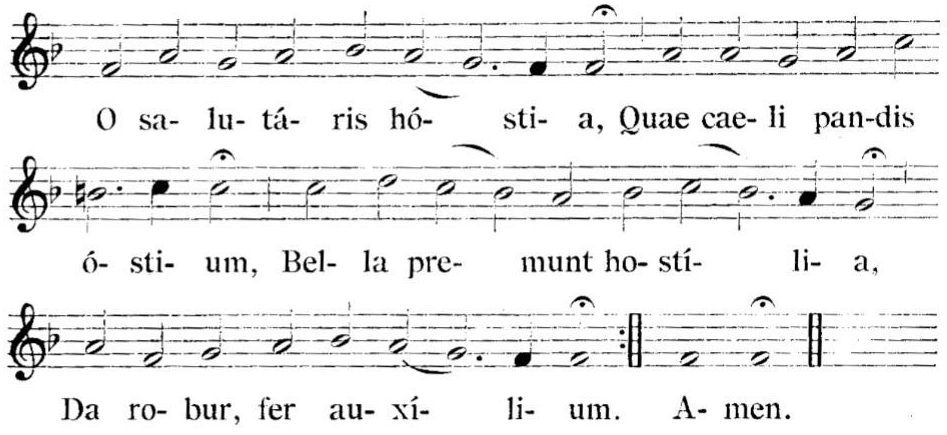
\includegraphics[width=\linewidth]{../ordinaires/o-salutaris.jpg}
  \end{figure}

  \begin{center}
    \begin{footnotesize}
      \textit{
        Ô réconfortante
        Hostie, Qui nous
        ouvres les portes du
        ciel, les armées ennemies
        nous poursuivent,
        Donne-nous la force,
        porte-nous secours.
      }
    \end{footnotesize}
  \end{center}

  \begin{multicols}{2}
    \begin{flushright}
      Uni trinoque Domino\\
      Sit sempiterna gloria :\\
      Qui vitam sine termino,\\
      Nobis donet in patria. Amen.\\
    \end{flushright}
    \columnbreak
    \textit{
      Au Seigneur unique en trois personnes,\\
      La gloire éternelle;\\
      qu'il nous donne en son Royaume\\
      La vie qui n'aura pas de fin. Amen\\
    }
  \end{multicols}

  \begin{center}
    \rule{2cm}{0.4pt}
  \end{center}

  \newpage

  % \begin{center}
  %   \textcolor{red}{\normalsize{Antienne à la Sainte Vierge.}}\\
  % \end{center}
  \begin{center}
    \textcolor{red}{\large{Salve Regína}}\\
    \begin{footnotesize}
      \textit{
      Du Dimanche de Pâques jusqu'au Vendredi après la Pentecôte inclusivement.
      }
    \end{footnotesize}
  \end{center}

  \gresetinitiallines{1}
  \greillumination{\initfamily\fontsize{11mm}{11mm}\selectfont S}
  \gregorioscore{an--salve_regina--solesmes}
  \medskip
  \begin{footnotesize}
    \textit{
      Salut, ô Reine, Mère de Miséricorde, notre vie, notre douceur, et notre espérance, salut. Vers vous nous élevons nos cris, pauvres exilés, malheureux enfants d'Eve. Vers vous nous soupirons, gémissant et pleurant dans cette vallée de larmes. De grâce donc, ô notre Avocate, tournez vers nous vos regards miséricordieux. Et, après cet exil, montrez-nous Jésus, le fruit béni de vos entrailles. Ô clémente, ô miséricordieuse, ô douce Vierge Marie.  
    }
  \end{footnotesize}

  \begin{multicols}{2}
    \parindent=0pt
    \begin{flushright}
      \textcolor{red}{\Vbar.} Ora pro nobis, Sancta Dei Génitrix.\\
      \textcolor{red}{\Rbar.} Ut digni efficiamur promissionibus Christi.\\
    \end{flushright}

    \columnbreak
    
    \textit{\textcolor{red}{\Vbar.} Priez pour nous, Sainte Mère de Dieu. \\
    \textcolor{red}{\Rbar.} Afin que nous soyons rendus dignes des promesses du Christ.}\\
  \end{multicols}

  \begin{multicols}{2}
    \parindent=0pt
    Omnípotens sempitérne Deus, qui gloriósæ Vírginis Matris Maríæ corpus et ánimam, ut dignum Fílii tui habitáculum effici mererétur, Spíritu Sancto cooperánte, præparásti : \textcolor{red}{†} da, ut, cujus commemoratióne lætámur, \textcolor{red}{*} ejus pia intercessióne, ab instántibus malis et a morte perpétua líberémur.\\ Per eúmdem Christum Dóminum nostrum.\\ 
    \textcolor{red}{\Rbar.} Amen.

    \columnbreak

    \textit{Dieu tout-puissant et éternel, qui avez préparé le corps et l’âme de la glorieuse Vierge et Mère Marie afin d’en faire une demeure digne de votre Fils, avec le concours du Saint-Esprit ; faites que, par la prière maternelle de celle dont nous évoquons avec joie la mémoire, nous soyons affranchis du mal présent et de la mort éternelle.\\
    Amen.
    }
  \end{multicols}

  \begin{center}
    \rule{2cm}{0.4pt}
  \end{center}

  \newpage

  \begin{center}
    \textcolor{red}{\large{En l'honneur Du Saint Sacrement}}
  \end{center}

  \gresetinitiallines{1}
  \greillumination{\initfamily\fontsize{11mm}{11mm}\selectfont T}
  \gregorioscore{../ordinaires/hy--tantum_ergo--solesmes}

  \begin{center}
    \begin{footnotesize}
      \begin{enumerate}[label=\textcolor{red}{\emph{\arabic*}}]
        \item \textit{Devant un sacrement si grand, prosternons-nous, adorons ; et que les symboles anciens s'effacent devant le rite nouveau ; que la foi vienne suppléer à la faiblesse de nos sens.}
        \item \textit{Au Père et au Fils louanges et acclamations, gloire honneur et puissance ainsi que bénédictions. A Celui qui de tous deux procède offrons une égale louange.}
      \end{enumerate}
    \end{footnotesize}
  \end{center}

  \medskip

  \begin{multicols}{2}
    \parindent=0pt
    \textcolor{red}{\Vbar.} Panem de caelo praestitisti eis.\\
    \textcolor{red}{\Rbar.} Omne delectamentum in se habentem.\\
    
    \textit{\textcolor{red}{\Vbar.} Tu leur a donné le pain du ciel.\\
    \textcolor{red}{\Rbar.} Toute saveur se trouve en lui.}\\
    
  \end{multicols}

  \bigskip

  \begin{center}
    \textcolor{red}{\large{Oraison}}
  \end{center}

  \begin{multicols}{2}
    \parindent=0pt
    Deus, qui nobis sub sacramento mirabili
    passionis tuæ memoriam reliquisti : \textcolor{red}{~†}
    tribue, quæsumus, ita nos Corporis et
    Sanguinis tui sacra mysteria venerari, \textcolor{red}{~*} ut
    redemptionis tuæ fructum in nobis
    jugiter sentiamus.\\
    Qui vivis et regnas
    cum Deo Patre in unitate Spiritus Sancti,
    Deus, per omnia sæcula sæculorum.
    Amen.
    \columnbreak

    \textit{
      Seigneur Jésus Christ, dans cet admirable
      sacrement tu nous a laissé le mémorial de
      ta passion ; donne-nous de vénérer d’un si
      grand amour le mystère de ton Corps et de
      ton Sang, que nous puissions recueillir
      sans cesse le fruit de ta rédemption. Toi
      qui règnes avec le Père et le Saint Esprit
      pour les siècles des siècles.
      Amen. 
    }
  \end{multicols}

  \begin{center}
    \rule{2cm}{0.4pt}
  \end{center}

  \newpage


  \begin{center}
    \textcolor{red}{\large{Louanges divines}}
  \end{center}


  \begin{normalsize}
    \parindent=0pt
    Dieu soit béni.\\
    Béni soit son Saint Nom.\\
    Béni soit Jésus-Christ, vrai Dieu et vrai homme.\\
    Béni soit le Nom de Jésus.\\
    Béni soit son Sacré Cœur.\\
    Béni soit son précieux Sang.\\
    Béni soit Jésus dans le très Saint Sacrement de l’autel.\\
    Béni soit l’Esprit Saint Consolateur.\\
    Bénie soit l’auguste Mère de Dieu, la très Sainte Vierge Marie.\\
    Bénie soit sa Sainte et Immaculée Conception.\\
    Bénie soit sa glorieuse Assomption.\\
    Béni soit le nom de Marie, Vierge et Mère.\\
    Béni soit Saint Joseph, son très chaste époux.\\
    Béni soit Dieu dans ses anges et dans ses saints.\\
    Seigneur, donnez-nous des prêtres.\\
    Seigneur, donnez-nous de saints prêtres.\\
    Seigneur, donnez-nous beaucoup de saints prêtres.\\
    Seigneur, donnez-nous beaucoup de saintes vocations religieuses.\\
  \end{normalsize}


  % \newpage

  \begin{center}
    \textcolor{red}{\large{Déposition}}\\
    \textit{Psaume 116}
  \end{center}

  \gresetinitiallines{1}
  \greillumination{\initfamily\fontsize{11mm}{11mm}\selectfont L}
  \gregorioscore{../temps_pascal/psaumes/ps--laudate_dominum_omnes_gentes_(psalmus_116)--solesmes}
  \bigskip
  \begin{footnotesize}
    \textit{
      Louez le Seigneur, tous les
      peuples ;
      Fêtez-Le, tous les pays !
      Son Amour envers nous
      S'est montré le plus fort ;
      Eternelle est la Fidélité du
      Seigneur !
      Gloire au Père, au Fils
      Et au Saint-Esprit,
      Comme il était au
      commencement,
      Maintenant et toujours,
      Pour les siècles des siècles,
      amen.
    }
  \end{footnotesize}

\end{document}